%===============================================================================
% LaTeX sjabloon voor de bachelorproef toegepaste informatica aan HOGENT
% Meer info op https://github.com/HoGentTIN/latex-hogent-report
%===============================================================================

\documentclass[dutch,dit,thesis]{hogentreport}

% TODO:
% - If necessary, replace the option `dit`' with your own department!
%   Valid entries are dbo, dbt, dgz, dit, dlo, dog, dsa, soa
% - If you write your thesis in English (remark: only possible after getting
%   explicit approval!), remove the option "dutch," or replace with "english".

\usepackage{lipsum} % For blind text, can be removed after adding actual content

%% Pictures to include in the text can be put in the graphics/ folder
\graphicspath{{graphics/}}

%% For source code highlighting, requires pygments to be installed
%% Compile with the -shell-escape flag!
\usepackage[section]{minted}
%% If you compile with the make_thesis.{bat,sh} script, use the following
%% import instead:
%% \usepackage[section,outputdir=../output]{minted}
\usemintedstyle{solarized-light}
\definecolor{bg}{RGB}{253,246,227} %% Set the background color of the codeframe

%% Change this line to edit the line numbering style:
\renewcommand{\theFancyVerbLine}{\ttfamily\scriptsize\arabic{FancyVerbLine}}

%% Macro definition to load external java source files with \javacode{filename}:
\newmintedfile[javacode]{java}{
    bgcolor=bg,
    fontfamily=tt,
    linenos=true,
    numberblanklines=true,
    numbersep=5pt,
    gobble=0,
    framesep=2mm,
    funcnamehighlighting=true,
    tabsize=4,
    obeytabs=false,
    breaklines=true,
    mathescape=false
    samepage=false,
    showspaces=false,
    showtabs =false,
    texcl=false,
}

% Other packages not already included can be imported here
\usepackage{parskip}
\def\code#1{\texttt{#1}}

%%---------- Document metadata -------------------------------------------------
% TODO: Replace this with your own information
\author{Anton Van Assche}
\supervisor{Dhr. T. Clauwaert}
\cosupervisor{Dhr. B. Deferme}
\title%
    {De identiteit van een Linux-systeem:\\ Onderzoek en Proof-of-Concept.}
\academicyear{\advance\year by -1 \the\year--\advance\year by 1 \the\year}
\examperiod{1}
\degreesought{\IfLanguageName{dutch}{Professionele bachelor in de toegepaste informatica}{Bachelor of applied computer science}}
\partialthesis{false} %% To display 'in partial fulfilment'
%\institution{Internshipcompany BVBA.}

%% Add global exceptions to the hyphenation here
\hyphenation{back-slash}

%% The bibliography (style and settings are  found in hogentthesis.cls)
\addbibresource{bachproef.bib}            %% Bibliography file
\addbibresource{../voorstel/voorstel.bib} %% Bibliography research proposal
\defbibheading{bibempty}{}

%% Prevent empty pages for right-handed chapter starts in twoside mode
\renewcommand{\cleardoublepage}{\clearpage}

\renewcommand{\arraystretch}{1.2}

%% Content starts here.
\begin{document}

%---------- Front matter -------------------------------------------------------

\frontmatter

\hypersetup{pageanchor=false} %% Disable page numbering references
%% Render a Dutch outer title page if the main language is English
\IfLanguageName{english}{%
    %% If necessary, information can be changed here
    \degreesought{Professionele Bachelor toegepaste informatica}%
    \begin{otherlanguage}{dutch}%
       \maketitle%
    \end{otherlanguage}%
}{}

%% Generates title page content
\maketitle
\hypersetup{pageanchor=true}

%%=============================================================================
%% Voorwoord
%%=============================================================================

\chapter*{\IfLanguageName{dutch}{Woord vooraf}{Preface}}%
\label{ch:voorwoord}

%% TODO:
%% Het voorwoord is het enige deel van de bachelorproef waar je vanuit je
%% eigen standpunt (``ik-vorm'') mag schrijven. Je kan hier bv. motiveren
%% waarom jij het onderwerp wil bespreken.
%% Vergeet ook niet te bedanken wie je geholpen/gesteund/... heeft

\lipsum[1-2]
%%=============================================================================
%% Samenvatting
%%=============================================================================

% TODO: De "abstract" of samenvatting is een kernachtige (~ 1 blz. voor een
% thesis) synthese van het document.
%
% Een goede abstract biedt een kernachtig antwoord op volgende vragen:
%
% 1. Waarover gaat de bachelorproef?
% 2. Waarom heb je er over geschreven?
% 3. Hoe heb je het onderzoek uitgevoerd?
% 4. Wat waren de resultaten? Wat blijkt uit je onderzoek?
% 5. Wat betekenen je resultaten? Wat is de relevantie voor het werkveld?
%
% Daarom bestaat een abstract uit volgende componenten:
%
% - inleiding + kaderen thema
% - probleemstelling
% - (centrale) onderzoeksvraag
% - onderzoeksdoelstelling
% - methodologie
% - resultaten (beperk tot de belangrijkste, relevant voor de onderzoeksvraag)
% - conclusies, aanbevelingen, beperkingen
%
% LET OP! Een samenvatting is GEEN voorwoord!

%%---------- Nederlandse samenvatting -----------------------------------------
%
% TODO: Als je je bachelorproef in het Engels schrijft, moet je eerst een
% Nederlandse samenvatting invoegen. Haal daarvoor onderstaande code uit
% commentaar.
% Wie zijn bachelorproef in het Nederlands schrijft, kan dit negeren, de inhoud
% wordt niet in het document ingevoegd.

\IfLanguageName{english}{%
\selectlanguage{dutch}
\chapter*{Samenvatting}
\lipsum[1-4]
\selectlanguage{english}
}{}

%%---------- Samenvatting -----------------------------------------------------
% De samenvatting in de hoofdtaal van het document

\chapter*{\IfLanguageName{dutch}{Samenvatting}{Abstract}}

Het onderwerp van cyberbeveiliging en de automatisering van systemen zijn beide van groot belang in de IT-wereld.
Toch is het samenvoegen van deze twee onderwerpen niet altijd vanzelfsprekend voor elk bedrijf.
Met de nieuwe NIS2-richtlijn, oftewel "Network and Information Security", worden bedrijven verplicht om hun systemen te beschermen tegen cyberaanvallen.
De reikwijdte van sectoren die onder deze richtlijn vallen, is aanzienlijk uitgebreid ten opzichte van zijn voorganger.
Een van de verplichtingen die bedrijven moeten nakomen, is het in kaart brengen van alle kritieke systemen die van invloed zijn op hun bedrijfsvoering.

Infrastructure as Code kan een oplossing bieden voor dit vraagstuk.
Door de huidige infrastructuur van een bedrijf te beschrijven in code, biedt het een overzicht van alle gebruikte systemen.
Toch vinden veel bedrijven, met name KMO's, het moeilijk om over te stappen naar een Infrastructure as Code omgeving.
Dit kan verschillende redenen hebben, zoals een gebrek aan kennis, tijd en budget.

Deze bachelorproef richt zich op het onderzoeken van mogelijke tools die kunnen helpen bij de overstap naar een Infrastructure as Code omgeving door het opstellen van een configuratie-inventaris.
Er zal worden gekeken naar bestaande tools die hieraan kunnen bijdragen.
Daarnaast zal er een analyse worden gemaakt van de verschillende eigenschappen van Linux-systemen die het beste kunnen worden opgenomen in een configuratie-inventaris.

Vervolgens zal er een Proof of Concept worden ontwikkeld, waarin een Bash-script zal worden geschreven dat basisinformatie van een Linux-systeem verzamelt en omzet in een verzameling van overzichtelijke bestanden.
Dit script zal worden uitgevoerd op vijf verschillende Debian servers, elk met hun eigen rol binnen de omgeving.

Deze bachelorproef verkent het gebruik van tools zoals Nmap en LinPEAS-ng voor het ontdekken van de configuratie van een Linux-systeem.
Nmap wordt voornamelijk ingezet voor het verkennen van netwerkconfiguraties, terwijl LinPEAS-ng dieper inzicht biedt in de configuratie van het Linux-systeem zelf en potentiële beveiligingsrisico's identificeert.
Het ontwikkelde script vormt een solide basis waarop beheerders kunnen voortbouwen door extra functionaliteiten toe te voegen en oplossingen te vinden voor eventuele beperkingen die tijdens de ontwikkeling van het script zijn geïdentificeerd.


%---------- Inhoud, lijst figuren, ... -----------------------------------------

\tableofcontents

% In a list of figures, the complete caption will be included. To prevent this,
% ALWAYS add a short description in the caption!
%
%  \caption[short description]{elaborate description}
%
% If you do, only the short description will be used in the list of figures

\listoffigures

% If you included tables and/or source code listings, uncomment the appropriate
% lines.
%\listoftables
%\listoflistings

% Als je een lijst van afkortingen of termen wil toevoegen, dan hoort die
% hier thuis. Gebruik bijvoorbeeld de ``glossaries'' package.
% https://www.overleaf.com/learn/latex/Glossaries

%---------- Kern ---------------------------------------------------------------

\mainmatter{}

% De eerste hoofdstukken van een bachelorproef zijn meestal een inleiding op
% het onderwerp, literatuurstudie en verantwoording methodologie.
% Aarzel niet om een meer beschrijvende titel aan deze hoofdstukken te geven of
% om bijvoorbeeld de inleiding en/of stand van zaken over meerdere hoofdstukken
% te verspreiden!

%%=============================================================================
%% Inleiding
%%=============================================================================

\chapter{\IfLanguageName{dutch}{Inleiding}{Introduction}}%
\label{ch:inleiding}

\section{\IfLanguageName{dutch}{Probleemstelling}{Problem Statement}}%
\label{sec:probleemstelling}

In het begin van 2023, op 6 januari, werd de NIS-richtlijn, wat staat voor "Network and Information Security", opgevolgd door zijn nieuwe versie, NIS2.
Deze update bracht verschillende nieuwe voorschriften met zich mee op het gebied van cyberbeveiliging, en het aantal sectoren dat aan deze richtlijnen moet voldoen, werd aanzienlijk uitgebreid.
Enkele sectoren die onder de NIS2 richtlijnen vallen zijn, maar niet beperkt tot~\autocite{NIS2Directive2022}:
\begin{itemize}
    \item Energie: elektriciteit, olie, gas, stadsverwarming en waterstof
    \item Transport: lucht, spoor, water en weg
    \item Digital infrastructuur: Telecom, DNS, TLD, datacenters, vertrouwensdiensten, clouddiensten, \ldots
    \item Digitale diensten: zoekmachines, online markten, sociale netwerken, \ldots
\end{itemize}

Het valt op dat de meeste sectoren die onder de NIS2-richtlijnen vallen, niet per se gericht zijn op IT.
Echter zijn bedrijven tegenwoordig in toenemende mate afhankelijk van bepaalde IT-processen die een impact hebben op hun bedrijfsvoering.
Dit maakt het noodzakelijk om ook cyberbeveiligingswetgevingen op hen toe te passen.

De lidstaten van de Europese Unie hebben tot oktober 2024~\autocite{NIS2Directive2022} de tijd om deze nieuwe richtlijnen in hun nationale wetgeving te implementeren.
Dit geeft bedrijven een beperkte periode om hun processen aan te passen aan deze nieuwe wetgeving, een uitdaging die vooral voor kleine of middelgrote ondernemingen (KMO's) problematisch kan zijn, gezien hun vaak beperkte middelen.

Een van de essenti\"ele vereisten van deze richtlijnen is dat bedrijven verplicht zijn om een ``inventory of assets'' op te stellen voor alle systemen en operaties die ze gebruiken.
Deze bachelorproef richt zich specifiek op het bieden van een oplossing voor KMO's, binnen sectoren die nu wel moeten voldoen aan deze richtlijnen, voor het inventariseren van Linux-systemen hun configuratie, waarbij de focus ligt op het vergemakkelijken van het naleven van deze nieuwe regelgeving.

Een manier die op dit moment veel gebruikt wordt om een inventaris van systemen en de configuratie ervan is het gebruik maken van Infrastructure as Code, ook wel IaC genoemd.
Het is een concept dat de laatste jaren steeds meer aan populariteit wint. Voornamelijk doordat het beheerders van computernetwerken in staat stelt om hun configuratie en infrastructuur vast te leggen in code, in plaats van handmatig te configureren.
Binnen deze code kunnen veelvoorkomende, complexe taken automatisch worden uitgevoerd, en dit alles op een geteste en foutloze manier~\autocite{chef-what-is-iac}.
Hier zullen we later verder op ingaan in hoofstuk~\ref{ch:stand-van-zaken}.

\section{\IfLanguageName{dutch}{Onderzoeksvraag}{Research question}}%
\label{sec:onderzoeksvraag}

\begin{enumerate}
    \item Hoe kunnen bedrijven, met name KMO's, zich aanpassen aan de nieuwe vereisten van de NIS2-richtlijn, met name met betrekking tot het opstellen van een ``inventory of assets'' voor hun IT-systemen?
    \item Op welke manieren kan Infrastructure as Code (IaC) worden ingezet om het inventariseren van systemen en configuraties te vergemakkelijken en te voldoen aan de eisen van de NIS2-richtlijn?
    \item Welke tools en technieken kunnen worden gebruikt om de configuratie en infrastructuur van Linux-systemen vast te leggen en te beheren?
    \item Welke configuratie-eigenschappen van Linux-systemen zijn essentieel om in kaart te brengen voor een inventaris?
\end{enumerate}

\section{\IfLanguageName{dutch}{Onderzoeksdoelstelling}{Research objective}}%
\label{sec:onderzoeksdoelstelling}

Het doel van deze bachelorproef is om een Proof of Concept te ontwikkelen die KMO's helpt bij het inventariseren van hun Linux-systemen en hun configuratie, met behulp van een Bash-script.
Het script zal rekening moeten houden met de bevindingen uit de risicoanalyse, en voorgaande hoofdstukken van deze bachelorproef.

Ook zal er een kritische evaluatie worden gemaakt van de Proof of Concept, waarbij de effectiviteit en volledigheid van de inventarisatie wordt beoordeeld.

\section{\IfLanguageName{dutch}{Opzet van deze bachelorproef}{Structure of this bachelor thesis}}%
\label{sec:opzet-bachelorproef}

% Het is gebruikelijk aan het einde van de inleiding een overzicht te
% geven van de opbouw van de rest van de tekst. Deze sectie bevat al een aanzet
% die je kan aanvullen/aanpassen in functie van je eigen tekst.

De rest van deze bachelorproef is als volgt opgebouwd:

In Hoofdstuk~\ref{ch:stand-van-zaken} wordt een overzicht gegeven van de stand van zaken binnen het onderzoeksdomein, op basis van een literatuurstudie.

In Hoofdstuk~\ref{ch:methodologie} wordt de methodologie toegelicht en worden de gebruikte onderzoekstechnieken besproken om een antwoord te kunnen formuleren op de onderzoeksvragen.

In Hoofdstuk~\ref{ch:linux-server-concepten} richten we ons op enkele fundamentele concepten van Linux-servers.

In Hoofdstuk~\ref{ch:computernetwerk-concepten} behandelen we de essenti\"ele concepten van computernetwerken in relatie tot servers.

In Hoofdstuk~\ref{ch:risicoanalyse} wordt een risicoanalyse uitgevoerd op de configuratie van Linux-servers, op basis van voorgaande hoofdstukken.

In Hoofdstuk~\ref{ch:poc} wordt een proof-of-concept uitgewerkt, waarbij de bevindingen van de risicoanalyse worden toegepast in een Bash-script.

In Hoofdstuk~\ref{ch:conclusie}, tenslotte, wordt de conclusie gegeven en een antwoord geformuleerd op de onderzoeksvragen. Daarbij wordt ook een aanzet gegeven voor toekomstig onderzoek binnen dit domein.

\chapter{\IfLanguageName{dutch}{Stand van zaken}{State of the art}}%
\label{ch:stand-van-zaken}

% Tip: Begin elk hoofdstuk met een paragraaf inleiding die beschrijft hoe
% dit hoofdstuk past binnen het geheel van de bachelorproef. Geef in het
% bijzonder aan wat de link is met het vorige en volgende hoofdstuk.

% Pas na deze inleidende paragraaf komt de eerste sectiehoofding.

\section{Network and Information Security 2}%
\label{sec:nis2}

\section{Huidige aanpak van asset management}%
\label{sec:huidige_aanpak_van_asset_management}

\subsection{Infrastructure as Code}%
\label{sub:iac}

Sinds de opkomst van computernetwerken is het uitrollen en beheren van servers en netwerken altijd een uitdagende taak geweest.
Infrastructure as Code (IaC) is een concept dat de laatste jaren steeds meer aan populariteit wint. Dit komt vooral doordat het beheerders van zulke netwerken in staat stelt om hun configuratie en infrastructuur vast te leggen in code, in plaats van handmatig te configureren.
Binnen deze code kunnen veelvoorkomende, complexe taken automatisch worden uitgevoerd, en dit alles op een geteste en foutloze manier~\autocite{chef-what-is-iac}.

IaC is gebaseerd op drie fundamentele concepten~\autocite{chef-what-is-iac}:
\begin{itemize}
    \item Automatisering: Het aanpassen van handmatige configuratie en het uitrollen van nieuwe servers worden allemaal geautomatiseerd met behulp van code.
    \item Testen: IT en DevSecOps processen kunnen met vertrouwen worden uitgevoerd omdat de code getest is.
    \item Idempotentie: Processen worden niet alleen toegepast op nieuwe servers, maar ook op bestaande servers om een consistente configuratie te behouden.
\end{itemize}

E\'en van de grootste voordelen van Iac is de verhoging van de effici\"entie~\autocite{splunk-benefits-iac}.
Doordat veel taken geautomatiseerd worden, kunnen beheerders zich richten op andere, meer complexe taken.
Zo heeft Red Hat in 2016 een casestudy gepubliceerd~\autocite{case-study-nasa-iac} waarin ze NASA's resultaten van hun overstap naar de IaC-tools Ansible en Ansible Tower hebben geanalyseerd.
Hierin geven ze aan dat het updateproces van nasa.gov van meer dan 1 uur is teruggebracht tot minder dan 5 minuten.
Het langdurige proces van het patchen van updates werd teruggebracht van een proces dat meerdere dagen in beslag nam naar een proces van ongeveer 45 minuten.

Het Duitse Federaal Ministerie van Voedsel en Landbouw (Bundesanstalt f\"ur Landwirtschaft und Ern\"ahrung, of BLE), heeft ook bepaalde IT-toepassingen met 50\% kunnen versnellen dankzij een overstap naar een IaC-aanpak~\autocite{case-study-ble-iac}.
In de studie bespreken ze kort waarom ze hebben besloten over te schakelen naar een IaC-aanpak en geven ze een paar voorbeelden van hoe ze voorheen te werk gingen en hoe ze dit met IaC hebben aangepakt.
Tijdens de implementatie hebben ze 1000 virtuele machines overgeschakeld van Debian en SUSE Linux naar Red Hat Enterprise Linux, ook bekend als RHEL.
Deze machines worden beheerd met behulp van Satellite en geautomatiseerd met Ansible.

Condition assessments is één van de belangrijkste componenten van IT asset management (IAM)~\autocite{ibm-what-is-iam}.
Dit proces houdt in dat men op elk moment de huidige staat kan bekijken van een asset.
Doordat IaC de configuratie van een asset vastlegt in code en zorgt dat deze consistent is, kan IaC ondersteuning bieden bij dit proces.

\subsection{Data Center Infrastructure Management}
\label{sub:dcim}

\subsection{IP Address Management}
\label{sub:ipam}

\subsection{Snipe-IT}
\label{sub:snipe-it}

Snip-IT is een open-source webapplicatie ontwikkeld door Grokability sinds 2013~\autocite{snipe-it-introduction}, die gericht is op IT-assetmanagement.
Het idee achter Snipe-IT komt voort uit de vroegere aanpak van het bedrijf, toen het voornamelijk nog gebruik maakte van spreadsheets om hun bedrijfsmiddelen te inventariseren.
Het doel was om een applicatie te ontwikkelen die deze taak op een meer georganiseerde en effici\"ente manier kon uitvoeren.

\begin{figure}[h!]
    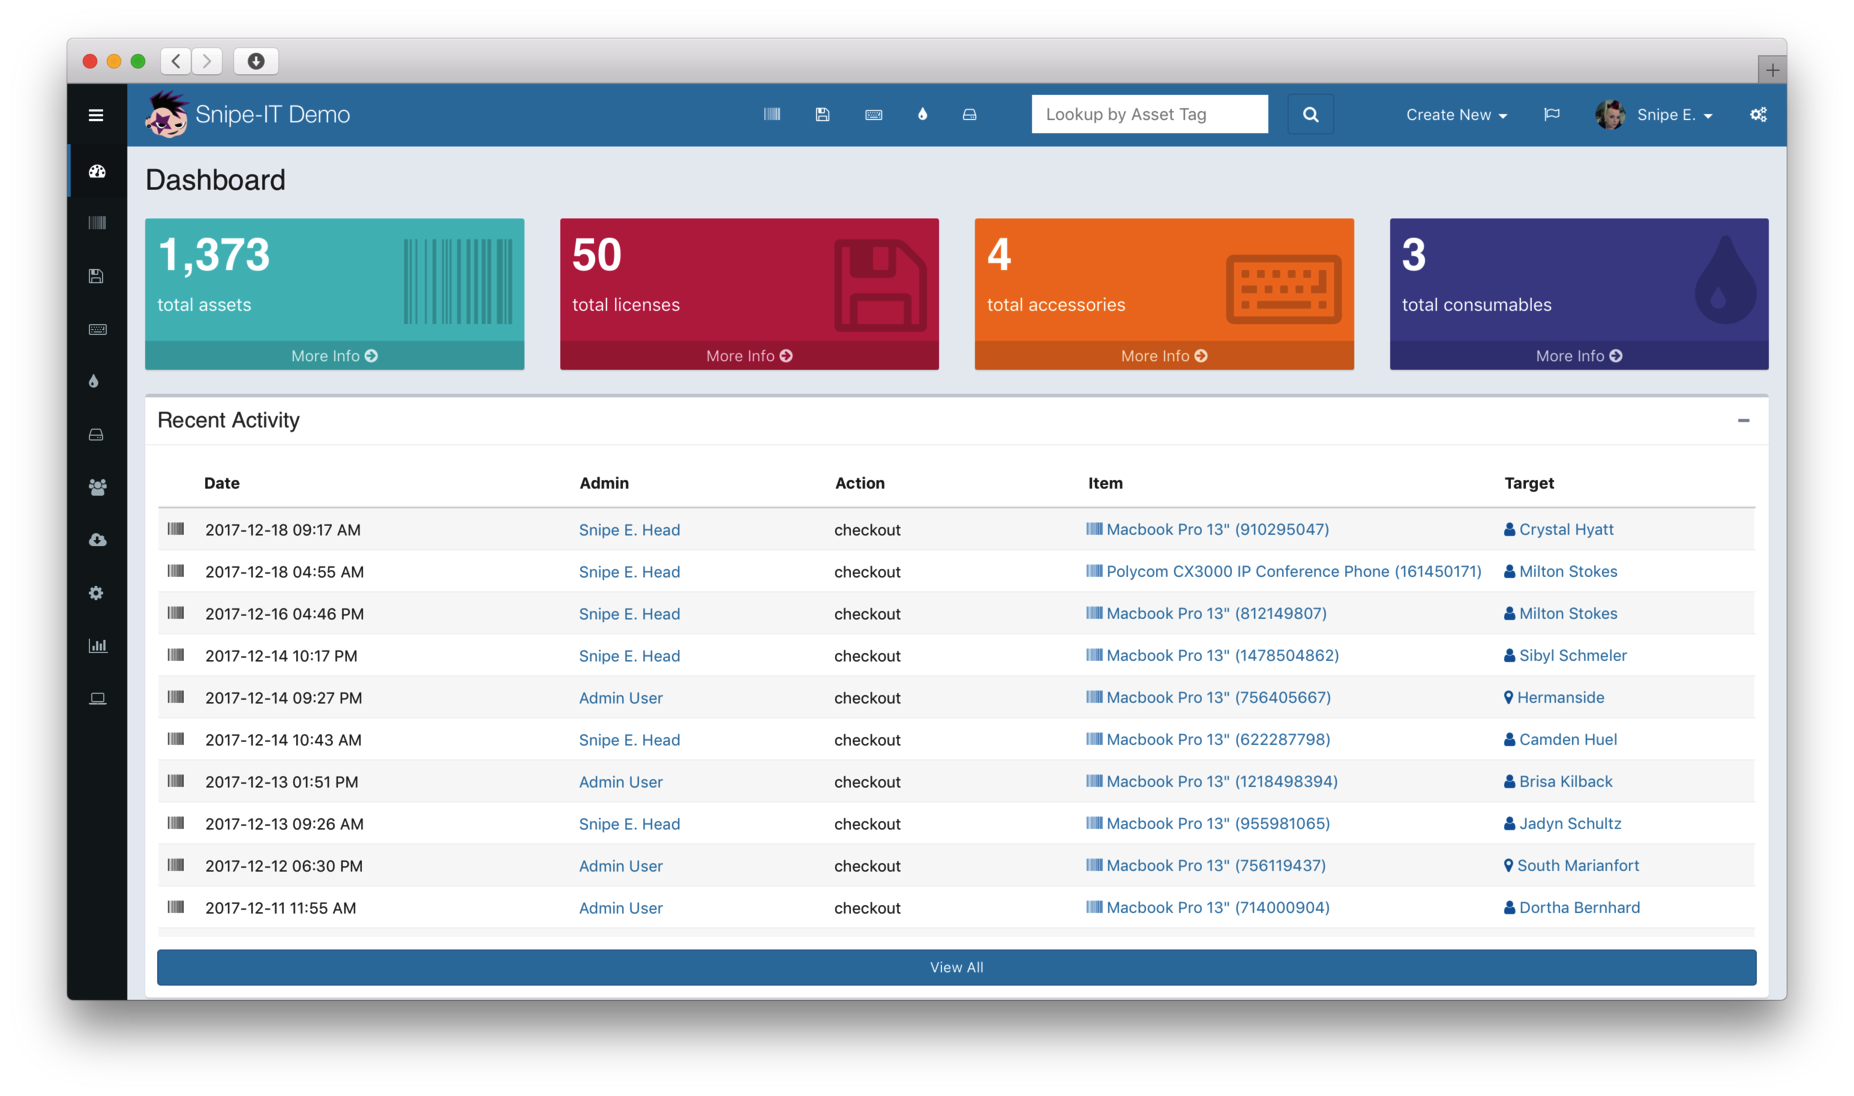
\includegraphics[width=\textwidth]
    {./graphics/snipe-dashboard.png}
    \caption{\label{fig:snipe-it-dashboard}Snip-IT dashboard waarin we het totale aantal assets binnen de organisatie kunnen zien, alsook een oplijsting van verschillende toestellen recent toegekend zijn~\autocite{snipe-it-dashboard}.}
\end{figure}

De software biedt een gebruiksvriendelijke webinterface (\ref{fig:snipe-it-dashboard}) waarmee bedrijfsmiddelen, licenties, garanties en meer gemakkelijk kunnen worden beheerd.
Wanneer men kiest voor de self-hosted optie is de software gratis beschikbaar, terwijl ook verschillende cloud-gebaseerde optie beschikbaar zijn tegen een jaarlijkse bijdrage.
Deze prijs varieert afhankelijk van de nodige features en support.
Alle code en services gerelateerd aan Snipe-IT zijn vrij beschikbaar op GitHub~\autocite{snipe-it-github}.

Enkele van de belangrijkste functies van Snipe-IT zijn~\autocite{snipe-it-features}, maar zijn niet beperkt tot:
\begin{itemize}
    \item Gemakkelijk zien welke assets zijn toegewezen, aan wie, en hun fysieke locatie
    \item In één klik inchecken
    \item Assetmodellen waarmee je gemeenschappelijke functies kunt groeperen
    \item Vereisen van Gebruikersacceptatie (Eindgebruikers EULA's/Gebruiksvoorwaar-\ den) bij Uitchecken
    \item E-mailmeldingen voor het verlopen van garanties en licenties
    \item Integratie met de meeste handheld barcode scanners en QR-codelezer apps
    \item Snelle en eenvoudige asset-audit
    \item Voeg je eigen aangepaste velden toe voor extra assetattributen
    \item Assets gemakkelijk importeren en exporteren
    \item Genereer QR-code labels voor eenvoudige mobiele toegang en labeling
    \item Assets gemarkeerd als aanvraagbaar kunnen worden aangevraagd door een gebruiker
    \item Assets behouden een volledige geschiedenis inclusief uitchecken, inchecken en onderhoud
    \item Optionele digitale handtekeningen bij assetacceptatie
\end{itemize}

\subsection{Nagios}
\label{sub:nagios}

\subsection{Lansweeper}
\label{sub:lansweeper}

Lansweeper, opgericht in 2004, is een Belgisch commercieel IT discovery \& inventory platform~\autocite{lansweeper-history}.
Het is een veelgebruikte tool voor het scannen, bijhouden en beheren van IT-assets binnen een organisatie.
Met functionaliteiten voor zowel hardware- als software-inventarisatie, biedt Lansweeper gebruikers een uitgebreid overzicht van alle IT-assets in hun netwerk.

Het grote voordeel van Lansweeper ten opzichte van andere tools, zoals Snipe-IT, is dat het een volledig geautomatiseerde oplossing biedt~\autocite{lansweeper-features}.
Dit betekent dat het platform in staat is om automatisch alle IT-assets binnen een netwerk te detecteren, zonder handmatige configuratie of de noodzaak om op elk systeem een agent te installeren~\autocite{lansweeper-getting-started}.
Een scan zal essenti\"ele informatie verzamelen over het asset, zoals de versie van het besturingssysteem, de hostname van de machine, het MAC-adres en de laatst ingelogde gebruiker.
Dit gebeurt met behulp van verschillende protocollen, waaronder SNMP.
De gedetecteerde informatie wordt vervolgens opgeslagen in een centrale database en is toegankelijk via een gebruiksvriendelijke webinterface.

\begin{figure}[h!]
    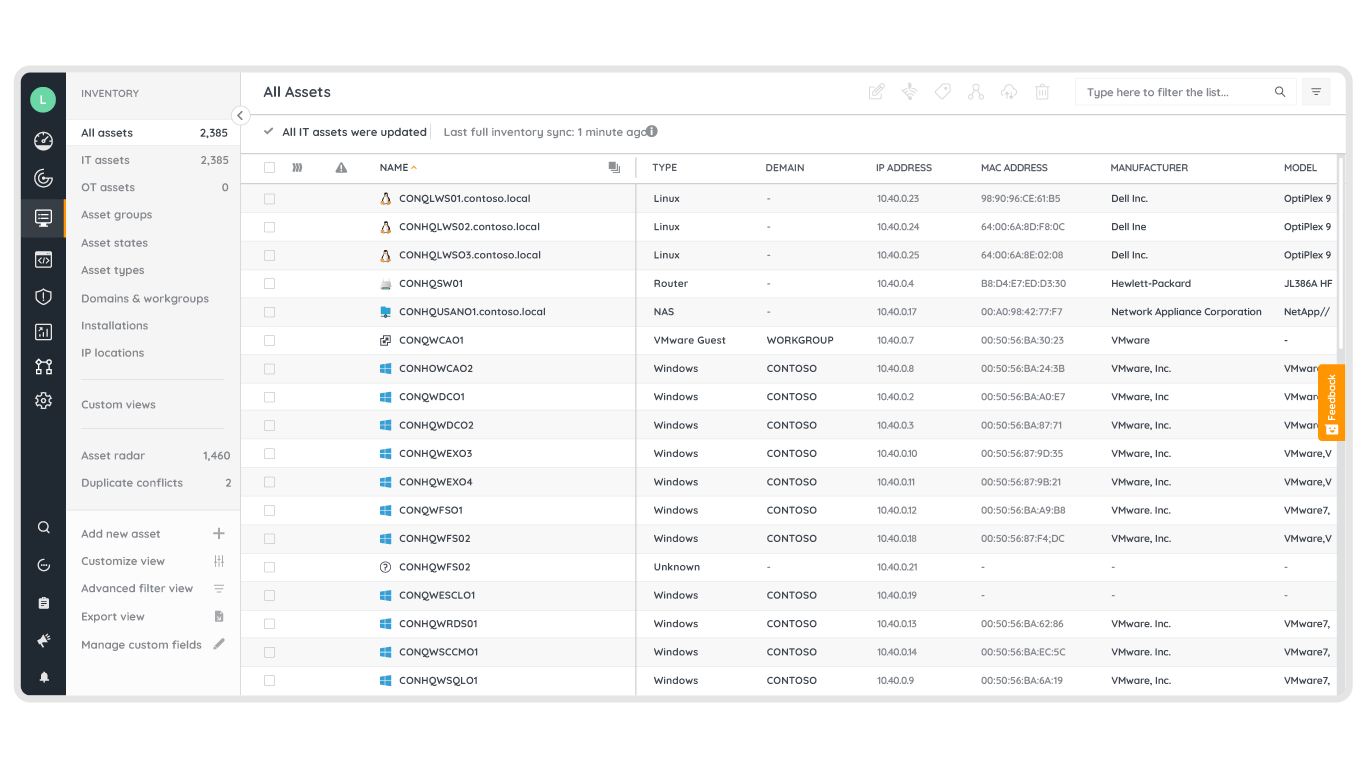
\includegraphics[width=\textwidth]
    {./graphics/lansweeper-dashboard.png}
    \caption{\label{fig:lansweeper-dashboard}Lansweeper dashboard.}
\end{figure}

Gebruikers kunnen aangepaste rapporten genereren over verschillende aspecten van hun IT-infrastructuur, zoals hardwareconfiguraties, softwarelicenties, patchniveaus en meer~\autocite{lansweeper-features}.
Deze rapporten zijn bruikbaar voor audits, nalevingscontroles en capaciteitsplanning.

Naast het genereren van rapporten en het identificeren van nieuwe IT-assets, biedt Lansweeper ook de mogelijkheid om rogue devices op het netwerk te detecteren.
Deze detectie gebeurt door continu het netwerk te scannen en alle gevonden assets te vergelijken met de resultaten in de database van bekende assets.
Wanneer een apparaat wordt gedetecteerd dat niet voorkomt in de database, genereert Lansweeper een waarschuwing, waardoor beheerders en administrators actie kunnen ondernemen.
Bovendien heeft Lansweeper de capaciteit om mogelijke beveiligingsrisico's te identificeren binnen uw inventaris door gebruik te maken van de NIST National Vulnerability Database~\autocite{lansweeper-cam}.

%%=============================================================================
%% Methodologie
%%=============================================================================

\chapter{\IfLanguageName{dutch}{Methodologie}{Methodology}}%
\label{ch:methodologie}

\section{Stand van zaken}
\label{sec:stand-van-zaken}
Dit onderdeel belicht de actuele benadering van configuration management, met een specifieke focus op Infrastructure as Code (IaC).
Naast een definitie van IaC worden de essenti\"ele componenten ervan besproken, evenals de voordelen die het met zich meebrengt.
Bovendien worden tools genoemd die kunnen worden ingezet om de configuratie van een systeem te identificeren en later om te zetten naar een IaC-omgeving.

Daarnaast zal er ook aandacht worden besteed aan asset management en hoe dit kan helpen bij de overgang van een niet-IaC-omgeving naar een IaC-omgeving.
Hoewel asset management minder gericht is op de configuratie van individuele machines, biedt het wel inzicht in de infrastructuur en de assets die beheerd moeten worden.
Op basis van deze informatie kunnen vervolgens de initi\"ele configuraties worden vastgelegd in code,

\section{Linux Server Concepten}
\label{sec:linux-server-concepten}
Dit hoofdstuk richt zich op de fundamentele concepten van Linux-servers.
Het doel is om een dieper begrip te bieden van de verschillende componenten en functies van een Linux-systeem, evenals de relevante ondersteunende tools.
Door deze basisbegrippen te verkennen, kunnen we effectiever bepalen welke informatie moet worden opgenomen in onze configuratie-inventaris.

\section{Computernetwerk Concepten}
\label{sec:computernetwerk-concepten}
Dit hoofdstuk behandelt de essenti\"ele concepten van computernetwerken in relatie tot servers.
We zullen verkennen hoe netwerkconnectiviteit een integraal onderdeel is van de functionaliteit van servers en hoe verschillende concepten en technologie\"en worden toegepast om deze connectiviteit te realiseren.

\section{Het opstellen van een configuratie-inventaris}
\label{sec:risicoanalyse}
In dit hoofdstuk zullen we een risicoanalyse uitvoeren voor Linux-systemen.
We zullen de bevindingen uit de eerdere hoofdstukken combineren om een lijst van cruciale configuratie-eigenschappen te presenteren voor het beheer en de beveiliging van Linux-systemen.
Door gebruik te maken van literatuuronderzoek en de besproken concepten, zullen we de risico's identificeren waaraan Linux-systemen blootstaan en welke specifieke eigenschappen moeten worden opgenomen in onze configuratie-inventaris.

\section{Proof of Concept}
\label{sec:proof-of-concept}
Dit hoofdstuk omvat de praktische toepassing van onze bevindingen.
We zullen een Bash-script ontwikkelen en uitvoeren op 5 virtuele Debian-servers, elk met hun eigen unieke taken en eigenschappen.
Dit stelt ons in staat om de bruikbaarheid en effectiviteit van onze aanpak te testen in een real-world scenario.

We zullen ook de gevonden resultaten analyseren en beoordelen of de configuratie-inventaris voldoet aan de verwachtingen en of deze als basis kan dienen voor een Infrastructure as Code (IaC)-omgeving.
Dit wordt gedaan door de resultaten te vergelijken met de bevindingen uit de risicoanalyse en de configuratie-inventaris.

%%=============================================================================
%% Proof of Concept
%%=============================================================================

\chapter{\IfLanguageName{dutch}{Proof of Concept}{Proof of Concept}}
\label{ch:poc}

\section{Inleiding}
\label{poc_inleiding}

In de vorige hoofdstukken hebben we uitgebreid de vereisten besproken die nodig zijn voor een doeltreffende configuratie-inventaris.
Nu is het tijd om deze vereisten in de praktijk te brengen door middel van een Proof of Concept (PoC).
In dit hoofdstuk zullen we ons richten op de praktische implementatie van deze vereisten.

We beginnen met het opzetten van de omgeving, waarbij we de technologie\"en toelichten die we zullen gebruiken om onze omgeving te automatiseren.
Vervolgens ontwikkelen we een Bash-script genaamd ConfiScan, dat dient om de configuratie-inventaris te genereren voor elke server binnen de omgeving.

Aan het einde van het hoofdstuk zullen we de resultaten van onze PoC presenteren.
Hierbij zullen we dieper ingaan op de functionaliteit en effectiviteit ervan.
Bovendien is alle bijbehorende code van deze Proof of Concept beschikbaar als open-source, te vinden op GitHub~\autocite{github-poc}.
Dit om de lezer de mogelijkheid te geven om de PoC zelf te testen en te gebruiken, en verder onderzoek mogelijk te maken.

\section{Beperkingen}
\label{poc_beperkingen}

De Proof of Concept (PoC) in deze bachelorproef heeft enkele beperkingen om de scope van het onderzoek te beheersen.
Primair is ervoor gekozen om de PoC te beperken tot enkel het gebruik van Debian als besturingssysteem.
Dit besluit is genomen omdat Debian een veelgebruikte distributie is in de serverwereld, die standaard wordt geleverd met een minimale set aan ge\"installeerde software en configuratie.
Hierdoor biedt het een ideale basis voor het onderzoeken van configuratie-inventaris.

Een andere beperkingen is dat beveiligingsmaatregelen zoals AppArmor en SELinux niet standaard ge\"installeerd zijn op Debian.
Deze zijn dan ook niet aanwezig op de virtuele machines die worden gebruikt voor de PoC.
Dit betekent dat het onderzoek zich voornamelijk zal richten op de standaardconfiguratie van Debian en de inventarisatie van de basisconfiguratie-instellingen.
Hoewel deze beperking de reikwijdte van het onderzoek verkleint, biedt het toch waardevolle inzichten in het proces van configuratie-inventarisatie binnen een specifieke context.

\section{Doelstellingen}
\label{poc_doelstellingen}

Het doel van deze Proof of Concept (PoC) is om een script te ontwikkelen en uit te voeren op de servers, dat de basisconfiguratie verzamelt zoals beschreven in hoofdstuk~\ref{ch:risicoanalyse}, en deze op één centrale locatie plaatst.
Het script zal worden ontworpen om de verschillende eigenschappen van de servers te verzamelen, waaronder netwerkconfiguraties, gebruikers- en groepsinformatie, ge\"installeerde software en andere relevante configuratie-instellingen.

Het is van cruciaal belang dat de verzamelde eigenschappen beschikbaar worden gesteld op een manier die eenvoudig te verwerken is, zoals CSV, JSON en tekstbestanden.
Dit zal het analyseren en verwerken van de verzamelde gegevens vergemakkelijken, en het mogelijk maken om rapporten te genereren en trends te identificeren binnen de configuratie van de servers.
Dit vergemakkelijkt mogelijks verder onderzoek dat kan volgen op deze bachelorproef.

Daarnaast zal het script ook de mogelijkheid moeten bieden om de configuratie van de ge\"installeerde software te kopi\"eren die relevant is voor de rol van de server en deze mee op te slaan in de centrale locatie.
Op deze manier kunnen we niet alleen de basisconfiguratie van de servers verzamelen, maar ook de specifieke configuratie-instellingen van de software die op elke server is ge\"installeerd.

Het uiteindelijke doel van deze PoC is om een voorbeeld te bieden om op een geautomatiseerde en gestructureerde manier de configuratie van meerdere servers te verzamelen en te beheren.
Door gebruik te maken van een script dat de configuratiegegevens centraliseert en eenvoudig toegankelijk maakt, kunnen we het beheer en de monitoring van onze serveromgeving verbeteren en effici\"enter maken.

\section{De omgeving}
\label{poc_omgeving}

Om de Proof of Concept uit te voeren, is het noodzakelijk om een virtuele omgeving te cre\"eren die een representatieve setting biedt voor het testen en evalueren van de configuratie-inventaris.
Dit proces omvat verschillende stappen, waaronder het opzetten van virtuele machines, het toewijzen van specifieke rollen aan elke server en het configureren van het netwerk om communicatie tussen de servers mogelijk te maken.

\subsection{Gekozen technologie{\"e}n}
\label{poc_gekozen_technologieen}

Om de omgeving zo reproduceerbaar mogelijk te maken, zullen we gebruik maken van verschillende technologie\"en die het opzetten van de omgeving automatiseren.
Dit stelt ons in staat om snel en consistent virtuele machines te cre\"eren en te configureren, wat essentieel is voor een succesvolle uitvoering van de Proof of Concept.

Allereerst zullen we gebruik maken van Vagrant~\autocite{vagrant-home}, in combinatie met VirtualBox~\autocite{virtualbox-home}, om de virtuele machines te beheren die de servers zullen vertegenwoordigen binnen deze PoC.
Vagrant biedt een eenvoudige en krachtige manier om virtuele machines te cre\"eren, te provisioneren en te beheren, waardoor we snel en effici\"ent onze testomgeving kunnen opzetten en terug afbreken tijdens het testen van de code.

Daarnaast zullen we Ansible~\autocite{ansible-home} gebruiken om elke server individueel te configureren en zijn specifieke rol binnen de omgeving te vervullen.
Ansible is een krachtige IaC-tool die ons in staat stelt om complexe configuratietaken uit te voeren met behulp van eenvoudig te begrijpen YAML-bestanden~\autocite{ansible-docs-yaml}.
Met Ansible kunnen we de configuratie van elke server nauwkeurig defini\"eren en consistent toepassen, wat bijdraagt aan de betrouwbaarheid en reproduceerbaarheid van onze omgeving.
Dit doordat dit een van de fundamenten is van IaC, zoals besproken in~\ref{sub:iac}.

\subsection{Serverrollen}
\label{poc_serverrollen}

De opgezette omgeving zal bestaan uit zes servers, waarvan vijf servers worden toegewezen aan verschillende serverrollen die we willen inventariseren, en één server zal fungeren als de centrale locatie voor de configuratie-inventaris en als de controller voor de servers.
In dit gedeelte zullen we de diverse rollen van de servers bespreken, evenals de gebruikte software om deze rollen te vervullen.

De keuze voor de serverrollen is tot stand gekomen in samenwerking met de co-promotor van deze bachelorproef, en deze rollen vertegenwoordigen een representatieve set van servers die vaak in de praktijk worden ingezet.
Dit zorgt ervoor dat onze PoC een breed scala aan serverconfiguraties kan omvatten en ons in staat stelt om een grondige inventarisatie uit te voeren van de configuratie-instellingen die relevant zijn voor elk type server.

Alvast een overzicht van de verschillende servers die deel zullen uitmaken van de omgeving, samen met de rol is te vinden in tabel~\ref{table:poc-server-roles}.

\begin{table}[!h]
    \begin{center}
        \begin{tabular}{ c c c }
            \hline
                Servernaam & IP-adres & Rol \\ [0.5ex]
            \hline
            control & 172.16.128.253 & Ansible-controller \\
            srv1    & 172.16.128.1   & DNS-server \\
            srv2    & 172.16.128.2   & Webserver \\
            srv3    & 172.16.128.3   & Database-server \\
            srv4    & 172.16.128.4   & Monitoring-server \\
            srv5    & 172.16.128.5   & Fileserver \\
        \end{tabular}
    \end{center}
    \caption{Overzicht van de verschillende rollen die worden toegewezen aan elke server binnen de omgeving.}
    \label{table:poc-server-roles}
\end{table}


\subsubsection{Ansible-controller}
\label{poc_ansible_controller}

De server met de naam \texttt{control} heeft de rol om de configuratie van de andere servers binnen de omgeving te beheren met behulp van Ansible.
We zullen deze server gebruiken om via Ansible het Bash-script uit te voeren op elke server.
Dit stelt ons in staat om de nodige bestanden met betrekking tot de configuratie-inventaris te verzamelen en te centraliseren op \'e\'en locatie.

\subsubsection{DNS-server}
\label{poc_dns_server}

De eerste server zal de rol van DNS-server binnen de omgeving vervullen.
Hiervoor zullen we gebruikmaken van de BIND DNS-server~\autocite{bind-home}, een van de meest gebruikte DNS-servers in de serverwereld.

Deze server zal een DNS-zone bevatten voor het domein \texttt{poc.lan}, waarbij de server zelf fungeert als de primaire nameserver voor deze zone.\
Hierdoor zal het gecentraliseerde DNS-informatie bevatten voor de andere servers binnen de omgeving, zoals IP-adressen en hostnamen.
Dit stelt ons in staat om de servers te bereiken via hun fully-qualified domain name (FQDN), in plaats van alleen hun IP-adres.
Bijvoorbeeld, we kunnen \texttt{srv1.poc.lan} gebruiken om de eerste server te bereiken, in plaats van \texttt{172.16.128.1}, dat het IP-adres van de DNS-server zelf zou zijn.

Wanneer een DNS-query niet kan worden beantwoord door de DNS-server zelf, zal deze worden doorgestuurd naar de DNS-server van de ISP.
Dit wordt mogelijk gemaakt door gebruik te maken van de NAT-interface van VirtualBox, waarbij Google (\texttt{8.8.8.8}) of Cloudflare (\texttt{1.1.1.1}) als backup DNS-servers zullen fungeren.

\subsubsection{Webserver}
\label{poc_webserver}

De tweede server, met hostname \texttt{srv2}, zal de rol van webserver vervullen binnen de omgeving.
We hebben ervoor gekozen om een basis Apache-webserver~\autocite{apache-home} te installeren, die een geconfigureerde website zal tonen wanneer deze wordt bezocht via een webbrowser.
De website zal bestaan uit een eenvoudige PHP-pagina die de inhoud van de database, geconfigureerd op \texttt{srv3}, zal weergeven.

\subsubsection{Database-server}
\label{poc_database_server}

Op \texttt{srv3} wordt een MariaDB-databaseserver~\autocite{maria-home} ge\"installeerd, die een database zal hosten met meerdere tabellen en records.
Deze tabellen zullen worden aangemaakt en gevuld met gegevens door gebruik te maken van een SQL-script, ontwikkeld door Patrick Allaert en openbaar beschikbaar op GitHub~\autocite{github-sql-script}.

De server zal verkeer van alle hosts binnen het netwerk toestaan en zal een specifieke gebruiker genaamd \texttt{appuser} bevatten.
Deze gebruiker heeft toegang tot de database, genaamd \texttt{appdb}, en de bijbehorende tabellen.

\subsubsection{Monitoring-server}
\label{poc_monitoring_server}

De vierde server, met de naam \texttt{srv4}, zal de rol van monitoring-server vervullen binnen de omgeving.
Hierop wordt Prometheus~\autocite{prometheus-home} ge\"installeerd, een veelgebruikte monitoringtool die wordt ingezet om metrische gegevens te verzamelen en te visualiseren van diverse systemen en services.
Deze server wordt geconfigureerd om alle metrische gegevens van de andere servers binnen de omgeving te verzamelen en te presenteren.

Dit wordt mogelijk gemaakt door het installeren van Node Exporter~\autocite{node-exporter-home} op elke server.
Node Exporter exposeert de metrische gegevens van de servers aan Prometheus, waardoor deze gegevens kunnen worden verzameld en geanalyseerd.

\subsubsection{Fileserver}
\label{poc_fileserver}

De laatste server die een specifieke rol zal vervullen binnen de omgeving is de fileserver, met de naam \texttt{srv5}.
Op deze server wordt een Samba-fileserver~\autocite{samba-home} ge\"installeerd.
Deze Samba-server biedt een gedeelde directory aan, specifiek genaamd \texttt{/mnt/storage\_01}, die beschikbaar is voor de andere servers binnen de omgeving.

Bovendien wordt er een gebruiker genaamd \texttt{james} aangemaakt, die lid is van de \texttt{sudo}-groep.
Deze gebruiker krijgt toegang tot de Samba-share en kan bestanden zowel lezen als schrijven naar deze share.

Daarnaast wordt voor de gebruiker een specifieke \texttt{sudo}-regel ingesteld, waardoor hij het \texttt{apt}-commando kan uitvoeren zonder een wachtwoord in te voeren.

\section{Ontwerp en implementatie}
\label{poc_ontwerp_implementatie}

In dit gedeelte zullen enkele ontwerp keuzes worden besproken die zijn gemaakt tijdens de ontwikkeling van het script, en hoe deze keuzes hebben bijgedragen aan de functionaliteit en effectiviteit van de Proof of Concept.
Voor een gedetailleerd overzicht van hoe de Proof of Concept werd uitgevoerd op elke server, verwijzen we naar bijlage~\ref{ch:bijlage_poc_uitvoering}.

\subsection{Bourne Again Shell (Bash)}
\label{poc_bash}

De Bourne Again Shell (Bash)~\autocite{gnu-bash-home} is een veelgebruikte shell, ook wel command language interpreter genoemd, die oorspronkelijk is ontwikkeld door de Free Software Foundation onder het GNU-project.
Aanvankelijk bedacht als een krachtiger alternatief voor de standaard Bourne Shell (sh) op GNU/Linux-systemen, heeft Bash zich ontwikkeld tot een van de meest populaire shells in de Linux-wereld.
Het wordt vaak gebruikt voor het schrijven van scripts en het automatiseren van diverse taken.

Een van de sterke punten van Bash is de hoge mate van compatibiliteit met zijn voorganger, de Bourne Shell, terwijl het ook handige functies uit andere shells zoals de Korn Shell (ksh) en de C Shell (csh) heeft ge\"integreerd.

De veelzijdigheid van Bash maakt het een uitstekende keuze voor het schrijven van scripts die verschillende taken moeten uitvoeren, zoals het verzamelen van configuratiegegevens van een server.
In combinatie met andere krachtige tools zoals \texttt{awk} en \texttt{sed}, kan Bash worden gebruikt om specifieke gegevens uit bestanden te filteren, te verwerken en op een leesbare manier weer te geven, alsook het automatiseren van verschillende taken.

\subsection{Comma-Separated Values (CSV)}
\label{poc_functionaliteiten_csv}

Een van de doelstellingen is om de configuratie-informatie op een zo toegankelijk mogelijke manier weer te geven.
Daarom is ervoor gekozen om veel van deze configuratie-eigenschappen te presenteren in CSV-formaat, ook wel bekend als Comma-Separated Values.
Dit tekstformaat maakt het mogelijk om gegevens in tabelvorm weer te geven, waarbij elke rij een record vertegenwoordigt en de kolommen de eigenschappen van dat record bevatten.
De gegevens worden gescheiden door komma's en elke nieuwe regel markeert een nieuwe rij.
CSV is een veelgebruikt formaat dat is ontworpen voor het importeren en exporteren van gegevens tussen verschillende programma's~\autocite{wikipedia2024csv}.

Een voorbeeld van het gebruik van dit formaat is bij het overbrengen van gegevens van een database naar een spreadsheetprogramma zoals Microsoft Excel.
De meeste spreadsheetprogramma's kunnen CSV-bestanden importeren en exporteren~\autocite{wikipedia2024csv}.
Dit maakt het eenvoudig om basisconfiguratie, zoals netwerkinterfaces van een server, over te zetten naar een spreadsheetprogramma.

Daarnaast zullen ook gewone tekstbestanden worden gebruikt om gegevens op te slaan.
Dit is vooral het geval voor complexe informatie waarvoor CSV niet geschikt is en het gebruik van CSV de leesbaarheid zou verminderen.
Een voorbeeld hiervan zijn de firewallregels, die vaak complexe configuraties bevatten en beter kunnen worden weergegeven in een tekstbestand.
Het weergeven van deze informatie in CSV-formaat zou de leesbaarheid van de gegevens verminderen, wat we zoveel mogelijk willen vermijden.

\begin{listing}
  \begin{minted}[linenos,tabsize=4,breaklines]{console}
Unit,State,Preset
cups.path,enabled,enabled
abrt-journal-core.service,enabled,enabled
abrt-oops.service,enabled,enabled
abrt-vmcore.service,enabled,enabled
abrt-xorg.service,enabled,enabled
abrtd.service,enabled,enabled
accounts-daemon.service,enabled,enabled
akmods.service,enabled,enabled
auditd.service,enabled,enabled
avahi-daemon.service,enabled,enabled
[...]
  \end{minted}
  \caption{Voorbeeld van alle enabled systemd units op een server in CSV-formaat.}
  \label{lst:poc-network-csv}
\end{listing}

\subsection{Applicatie specifieke configuratie}
\label{poc_functionaliteiten_app_config}

Het script biedt ook een flexibele manier om de configuratie van specifieke applicaties op de servers te inventariseren, zoals vereist in de doelstellingen.
Voor deze bachelorproef is ervoor gekozen om de gebruiker zelf de configuratiebestanden of directories te laten kiezen en specificeren als argumenten bij het uitvoeren van het script.
Deze aanpak geeft de gebruiker de vrijheid om de configuratie van specifieke applicaties te selecteren die relevant zijn voor hun behoeften en omgeving.
Wanneer men geen specifieke configuratiebestanden of directories opgeeft, zal het script een kopie maken van de gehele \texttt{/etc}-directory, die de meeste configuratiebestanden bevat voor de ge\"installeerde software op de server.

Wanneer het script wordt uitgevoerd, kunnen gebruikers eenvoudig de gewenste configuratiebestanden of -directories opgeven als argumenten.
Zoals te zien is in listing~\ref{lst:poc-config-args}, wordt het script uitgevoerd met de configuratiebestanden van Apache en de SSH-daemon als argumenten.

\begin{listing}
  \begin{minted}[linenos,tabsize=4,breaklines]{console}
vagrant@srv1:~$ ./confiscan.sh /etc/apache2/apache2.conf /etc/ssh/sshd_config
  \end{minted}
  \caption{Voorbeeld van het uitvoeren van het script met specifieke configuratiebestanden als argumenten.}
  \label{lst:poc-config-args}
\end{listing}

\subsection{/proc-bestandssysteem}
\label{poc_functionaliteiten_proc}

Het \texttt{/proc}-bestandssysteem is een virtueel bestandssysteem dat kan worden beschouwd als een schat aan informatie over het systeem.
Het is een speciaal bestandssysteem dat Linux heeft ge\"erfd van zijn voorganger, UNIX, en dat een breed scala aan informatie bevat over de actieve processen, kernelmodules, hardwareconfiguratie en andere systeemgerelateerde gegevens.
Beheerd door de Linux-kernel zelf en vaak read-only voor reguliere gebruikers, kan het worden beschouwd als een bron van waarheid voor informatie over het systeem~\autocite{rhel-proc}.

\begin{listing}
  \begin{minted}[linenos,tabsize=4,breaklines]{console}
[anton@fedorable ~]$ cat /proc/sys/kernel/hostname
fedorable
  \end{minted}
  \caption{Voorbeeld van het weergeven van de hostname van de server.}
  \label{lst:poc-proc-hostname}
\end{listing}

Enkele handige bestanden binnen het \texttt{/proc}-bestandssysteem zijn, die ook zullen worden gebruikt in het script, zijn:

\begin{itemize}
    \item \texttt{/proc/sys/kernel/hostname}: Bevat de hostname van de server, zoals weer te geven in listing~\ref{lst:poc-proc-hostname}.
    \item \texttt{/proc/cmdline}: Bevat de boot parameters die zijn doorgegeven aan de kernel tijdens het opstarten.
    \item \texttt{/proc/modules}: Lijst van alle geladen kernel modules.
    \item \texttt{/proc/filesystems}: Lijst van alle bestandssystemen die door de kernel worden ondersteund.
    \item \texttt{/proc/mounts}: Lijst van alle actieve mount points op het systeem.
\end{itemize}

Tijdens deze Proof of Concept zullen we naast het verwerken van commando's ook informatie verzamelen uit dit virtuele bestandssysteem.
We zullen gegevens verzamelen over kernelmodules, actieve mount points en andere systeemgerelateerde informatie.
Vervolgens zullen we deze informatie verwerken en opslaan in de configuratie-inventaris in een leesbare vorm, zoals CSV- of tekstbestanden.

\section{De resultaten}
\label{poc_resultaten}

Tijdens de ontwikkelingsfase van het script hebben we rekening gehouden met de besproken onderwerpen uit hoofdstuk~\ref{ch:risicoanalyse}.
Hierdoor zijn we erin geslaagd om een script te ontwikkelen dat de configuratie-inventaris van een server kan genereren.
Na het uitvoeren van het script op elke server binnen de omgeving, hebben we voor elke server een directory met bestanden ontvangen die verschillende eigenschappen van de server bevatten.
Als de \texttt{-t} optie wordt gebruikt, wordt er een tarball gegenereerd van deze directory.
Dit maakte het eenvoudig om de configuratie-inventaris te verzamelen en te centraliseren op de controller-server, waar we de gegevens kunnen analyseren en verwerken.
Tabel~\ref{table:poc-inventory-properties} toont een algemeen overzicht van de eigenschappen die al dan niet zijn opgenomen in de configuratie-inventaris.

Uit de resultaten vermeld in tabel~\ref{table:poc-inventory-properties} kunnen we concluderen dat de meeste eigenschappen van de serverconfiguratie met succes zijn opgenomen in de configuratie-inventaris.
Echter zijn er enkele beperkingen, waaronder het ontbreken van de AppArmor- en SELinux-configuraties, die niet zijn opgenomen in de configuratie-inventaris.
Dit kan worden opgelost door de directory of configuratiebestanden van deze beveiligingsmaatregelen mee te geven als commandline-argumenten.
Dit zorgt ervoor dat de configuratiebestanden toch worden opgenomen in de confi-\ guratie-inventaris.

Een alternatieve aanpak is het toevoegen van een aparte sectie waarin we de configuratie van AppArmor en SELinux kunnen opnemen.
Indien gewenst kunnen deze gegevens dan worden omgezet naar een leesbaar formaat, zoals CSV of tekstbestanden.
Echter is ervoor gekozen om dit specifieke aspect niet in deze bachelorproef op te nemen, zowel om de scope te beperken als omdat Debian standaard geen AppArmor of SELinux ge\"installeerd heeft.

Een andere beperking heeft betrekking op het opnemen van specifieke softwareconfiguraties.
Wanneer een directory of bestand wordt meegegeven als argument, wordt dit letterlijk gekopieerd naar de configuratie-inventaris.
Dit houdt geen rekening met het soort bestand.
Als het bijvoorbeeld een softlink is, bestaat de kans dat deze niet zal werken na het inventariseren van de configuratie.
Dit werd vastgesteld tijdens het testen van het script op \texttt{srv2}, waar we de \texttt{my.cnf} van MariaDB wilden opnemen in de configuratie-inventaris.
Maar dit een softlink was naar \texttt{/etc/alternatives/my.cnf}, wat niet werd meegegeven als argument.

Wanneer het echter een softlink betreft naar een bestand binnen de gespecificeerde directory, zal deze wel blijven werken.
Dit werd bevestigd na het uitvoeren van het script op \texttt{srv3}, waarbij we succesvol de configuratie van Apache, inclusief de softlinks van de modules in \texttt{/etc/apache2/mods-enabled}, hebben opgenomen in de configuratie-inventaris.

\def\checkmark{\tikz\fill[scale=0.4](0,.35) -- (.25,0) -- (1,.7) -- (.25,.15) -- cycle;}
\begin{table}[!h]
    \begin{center}
        \begin{tabular}{ c c c }
            \hline
                Eigenschap & Opgenomen & Niet opgenomen \\ [0.5ex]
            \hline
                AppArmor                        &            & \checkmark \\
                BIOS-informatie                 & \checkmark &            \\
                Bestandssystemen                & \checkmark &            \\
                Besturingssysteem               & \checkmark &            \\
                Boot parameters                 & \checkmark &            \\
                CPU-informatie                  & \checkmark &            \\
                Cronjobs                        & \checkmark &            \\
                DNS-configuratie                & \checkmark &            \\
                Firewallregels                  & \checkmark &            \\
                Ge\"installeerde software       & \checkmark &            \\
                Gebruikers                      & \checkmark &            \\
                Geheugeninformatie              & \checkmark &            \\
                Groepen                         & \checkmark &            \\
                Kernelmodules                   & \checkmark &            \\
                Kernelversie                    & \checkmark &            \\
                Mount points                    & \checkmark &            \\
                Netwerkinterfaces               & \checkmark &            \\
                Partities                       & \checkmark &            \\
                Repositories                    & \checkmark &            \\
                Routingtabel                    & \checkmark &            \\
                SELinux                         &            & \checkmark \\
                Specifieke softwareconfiguratie & \checkmark &            \\
                Systeeminformatie               & \checkmark &            \\
                Systemd units                   & \checkmark &            \\
                TCP/UDP-poorten                 & \checkmark &            \\
                \text{sudo}-regels              & \checkmark &            \\
        \end{tabular}
    \end{center}
    \caption{Overzicht van de eigenschappen die al dan niet zijn opgenomen in de configuratie-inventaris.}
    \label{table:poc-inventory-properties}
\end{table}

De resultaten van het script zijn systematisch vergeleken met zowel de configuratie die door Ansible is toegepast op de servers als de daadwerkelijke configuratie van de servers zelf.
Aangezien het script de configuratie van de applicaties reproduceert, komen deze gegevens in de configuratie-inventaris overeen met de configuratie die door Ansible is toegepast.
Het implementeren van een file-integriteitscon-\ trole, zoals gedaan door het script met behulp van \texttt{sha256sum}, kan een extra laag van controle bieden om de integriteit van de configuratiebestanden te waarborgen.
Bovendien stelt het ons in staat om later eventuele wijzigingen in de configuratiebestanden te identificeren.
Wanneer we de resultaten van de configuratie die door Vagrant doorgevoerd werd bekijken, merken we op dat deze ook overeenkomen met de specificaties in het \texttt{vagrant-hosts.yml} bestand.
Deze resultaten betreffen voornamelijk de netwerkconfiguratie, zoals IP-adressen en hostnamen.

Over het algemeen biedt het script een solide basis voor verdere ontwikkeling en uitbreiding van de configuratie-inventaris met meer eigenschappen en functionaliteiten op Debian-servers.
Bijna elke beperking die tijdens het testen van het script is ge\"identificeerd, kan worden overwonnen door de functionaliteit van het script uit te breiden en te verbeteren.
Een mogelijke oplossing voor het probleem met softlinks is bijvoorbeeld het implementeren van een mechanisme dat de bestanden volgt en controleert of het al dan niet een link is.
Als het een link is, kan het script de link volgen en het gekoppelde bestand ook toevoegen aan de configuratie-inventaris.
Een alternatieve oplossing, waarbij gebruik wordt gemaakt van \texttt{rsync}, wordt behandeld in bijlage~\ref{ch:bijlage_symlink_kopieren_met_rsync}.

Bovendien kunnen we door het gebruik van bestandsformaten zoals CSV en tekstbestanden de verkregen resultaten eenvoudig visualiseren.
Dit kan worden gedaan met behulp van spreadsheetprogramma's of door het ontwikkelen van aangepaste applicaties voor verder onderzoek en analyse.

Een voorbeeld van de uitvoer van het script is te vinden in bijlage~\ref{ch:bijlage_confiscan}.


% Voeg hier je eigen hoofdstukken toe die de ``corpus'' van je bachelorproef
% vormen. De structuur en titels hangen af van je eigen onderzoek. Je kan bv.
% elke fase in je onderzoek in een apart hoofdstuk bespreken.

%\input{...}
%\input{...}
%...

%%=============================================================================
%% Conclusie
%%=============================================================================

\chapter{Conclusie}%
\label{ch:conclusie}

Deze bachelorproef had als doel het verkennen van het gebruik van Infrastructure as Code (IaC) om te voldoen aan de NIS2-eis voor het bijhouden van een ``inventory of assets''.
Specifiek lag de focus op het ontwikkelen van een praktische oplossing voor het opstellen van een configuratie-inventaris op Linux-systemen te automatiseren.

We begonnen met een diepgaande bespreking van de fundamentele principes van Infrastructure as Code, zoals idempotentie, automatisatie en testen.
Hierbij hebben we de voordelen van IaC onderzocht aan de hand van literatuurstudie, met speciale aandacht voor tools zoals Puppetboard die ervoor zorgen dat we direct een configuratie-inventaris hebben bij het gebruik van Puppet.

Tijdens de literatuurstudie hebben we ook gekeken naar verschillende tools die kunnen helpen bij het ontdekken van configuratie-eigenschappen van Linux-syste-\ men, zoals Nmap en linPEAS-ng.
Zo bleek dat Nmap reeds gebruikt wordt om netwerken in kaart te brengen, en dus ons kan helpen bij het verzamelen van netwerkconfiguratie, zoals het detecteren van open poorten binnen het netwerk als ook hosts te ontdekken.
LinPEAS-ng kan dan weer helpen bij het identificeren van gevoelige configuratie-eigenschappen zoals rechten van bestanden en gebruikers en is meer gericht in kwetsbaarheden te vinden in de configuratie van een systeem.

Daarnaast hebben we ook een blik geworpen op de huidige aanpak van asset management in de praktijk, waarbij tools zoals Snipe-IT, Lansweeper en NetBox werden onderzocht.
Deze tools zijn van belang voor het inventariseren van hardware, software, licenties en netwerkgerelateerde zaken.
Waar NetBox vooral gebruikt wordt voor het inventariseren van netwerkgerelateerde zaken zoals IP-adressen en VLAN's.

Vervolgens werd een risicoanalyse uitgevoerd om essenti\"ele configuratie-eigen-\ schappen van Linux-systemen te identificeren die moeten worden opgenomen in de configuratie-inventaris.
Hierbij hebben we gekeken naar factoren die de identiteit van een Linux-systeem bepalen, zoals het besturingssysteem, netwerkinterfaces, ge\"installeerde software en beveiligingsaspecten.

De resultaten van de risicoanalyse werden ge\"implementeerd in een Proof of Concept (PoC), waarbij het Bash-script genaamd ConfiScan werd ontwikkeld.
Dit script is specifiek ontworpen voor Debian-gebaseerde systemen en maakt gebruik van verschillende commando's en bestanden in \texttt{/proc/} om configuratie-eigenschap-\ pen te verzamelen en op te slaan in CSV- en tekstbestanden.

Het script werd uitvoerig getest op vijf virtuele machines met behulp van Vagrant en Ansible voor de configuratie.
Tijdens deze fase werden enkele beperkingen van het script ge\"identificeerd, zoals problemen met het correct verwerken van soft- en hardlinks die naar andere locaties verwijzen buiten het opgegeven pad.
Mogelijke oplossingen werden besproken, zoals het gebruik van \texttt{rsync}.

Ondanks deze beperkingen biedt het ontwikkelde script een solide basis voor verdere ontwikkeling en uitbreiding.
Toekomstige verbeteringen kunnen onder meer het volgen van soft- en hardlinks omvatten, evenals het toevoegen van specifieke functionaliteit voor het vastleggen van SELinux- of AppArmor-configuraties.

In de toekomst kan het script verder worden uitgebreid en ge\"integreerd in bestaande systeembeheerprocessen.
Ook kan het worden aangepast voor ondersteuning van andere besturingssystemen en cloudomgevingen, waardoor de bruikbaarheid ervan wordt vergroot.
Dit onderzoek draagt bij aan het vakgebied van systeembeheer en biedt een praktische oplossing voor het automatiseren van configu-\ ratie-inventarisatie op Linux-servers.


%---------- Bijlagen -----------------------------------------------------------

\appendix

\chapter{Onderzoeksvoorstel}

Het onderwerp van deze bachelorproef is gebaseerd op een onderzoeksvoorstel dat vooraf werd beoordeeld door de promotor. Dat voorstel is opgenomen in deze bijlage.

%% TODO:
%\section*{Samenvatting}

% Kopieer en plak hier de samenvatting (abstract) van je onderzoeksvoorstel.

% Verwijzing naar het bestand met de inhoud van het onderzoeksvoorstel
%---------- Inleiding ---------------------------------------------------------

\section{Introductie}%
\label{sec:introductie}

In het begin van 2023, op 6 januari, werd de NIS-richtlijn, wat staat voor "Network and Information Security", opgevolgd door zijn nieuwe versie, NIS2.
Deze update bracht verschillende nieuwe voorschriften met zich mee op het gebied van cyberbeveiliging, en het aantal sectoren dat aan deze richtlijnen moet voldoen, werd aanzienlijk uitgebreid.

De lidstaten van de Europese Unie hebben tot oktober 2024~\autocite{NIS2Directive2022} de tijd om deze nieuwe richtlijnen in hun nationale wetgeving te implementeren.
Dit geeft bedrijven een beperkte periode om hun processen aan te passen aan deze nieuwe wetgeving, een uitdaging die vooral voor kleine of middelgrote ondernemingen (KMO's) problematisch kan zijn, gezien hun vaak beperkte middelen.

Een van de essenti\"ele vereisten van deze richtlijnen is dat bedrijven verplicht zijn om een ``inventory of assets'' op te stellen voor alle systemen en operaties die ze gebruiken.
Deze bachelorproef richt zich specifiek op het bieden van een oplossing voor KMO's, binnen sectoren die nu wel moeten voldoen aan deze richtlijnen, voor het inventariseren van Linux-systemen hun configuratie, waarbij de focus ligt op het vergemakkelijken van het naleven van deze nieuwe regelgeving.

Om dit te bereiken, zal een script of tool worden ontwikkeld die automatisch op elke Linux-server kan worden uitgevoerd, en gekeken worden naar reeds bestaande oplossingen die we kunnen gebruiken.
Deze tool biedt vervolgens een gedetailleerde inventaris van het systeem en de configuratie van verschillende applicaties.
Het uiteindelijke doel is om deze tool uit te voeren op vijf verschillende servers met specifieke use cases.
Op basis hiervan zal worden geconcludeerd of het implementeren van deze tool nuttig is voor KMO's.

%---------- Stand van zaken ---------------------------------------------------

\section{Literatuurstudie}%
\label{sec:litaratuurstudie}

Volgens een studie uit 2022~\autocite{Kotenko2022} is het opstellen van een configuratie inventaris essentieel voor het beoordelen van cybersecurityrisico's.
Aan de hand van een inventaris kan men potenti\"ele kwetsbaarheden gaan identificeren en de passende maatregelen gaan treffen.
Ook wordt er benadrukt dat het inventaris kan gebruikt worden om mogelijke cyberaanvalspaden te identificeren en het voorkomen van verliezen door cyberaanvallen.
Het regelmatig herevalu\"eren van het inventaris wordt benadrukt als een proactieve benadering om potenti\"ele incidenten te voorkomen.
Dit benadrukt het belang van een nauwkeurige inventarisatie voor het implementeren van geautomatiseerde detectie- en bewakingsmaatregelen.

In een boek geschreven door Antal~\autocite{Antal2010} worden verschillende systeemeigenschappen genoemd die essentieel zijn voor een inventaris.
Hoewel het boek niet specifiek gericht is op Linux-systemen, biedt het een algemeen overzicht van cruciale aspecten van een inventaris.
Hierbij wordt de configuratie van het besturingssysteem benadrukt, inclusief details zoals de kernel- en besturingssysteemversie.
Verder wordt het belang van het aantal geïnstalleerde applicaties en hun configuratie benoemd als significant in het inventarisatieproces.
Daarnaast wordt de netwerkconfiguratie, waaronder IP-adressen en firewallconfiguratie, als essentieel beschouwd.

%---------- Methodologie ------------------------------------------------------
\section{Methodologie}%
\label{sec:methodologie}

In deze studie wordt onderzoek gedaan naar de bijdrage van een configuratie-inventaris van Linux-systemen aan het initi\"ele proces van incident response bij een cyberaanval.
Het onderzoek zal bestaan uit zes fasen, zoals weergegeven in figuur~\ref{fig:flowchart}.

\begin{figure}[h!]
    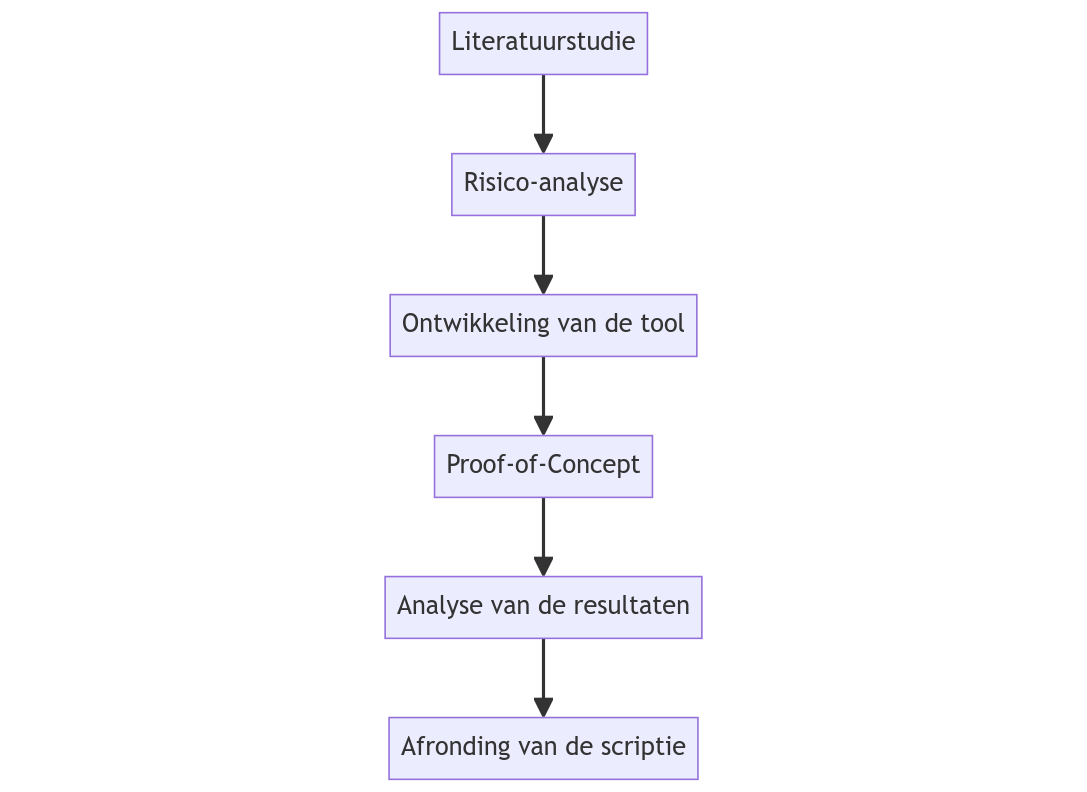
\includegraphics[width=.49\textwidth]
    {graphics/methodologie_flowchart.png}
    \caption{\label{fig:flowchart}Flowchart fasen methodologie}
\end{figure}


\subsection{Fase 1: Literatuurstudie}%
\label{sub:literatuurstudie}

De eerste fase omvat een grondige literatuurstudie die zich richt op het verzamelen van essenti\"ele configuratie en eigenschappen voor een grondig inventaris.
Daarnaast zullen ook bestaan\\de tools worden onderzocht die kunnen gebruikt worden bij het inventariseren van Linux-systemen.
Deze fase zal 2 weken in beslag nemen, en resulteert in een literatuurstudie die niet alleen de  eigenschappen van Linux-systemen identificeert die relevant zijn voor het inventaris, maar ook reeds bestaande tools die hiervoor gebruikt kunnen worden.

\subsection{Fase 2: Risico-analyse}%
\label{sub:risico_analyse}

De tweede fase richt zich op een risico-analyse, waarbij de ge\"identificeerde Linux-systeem\\eigenschappen binnen het inventaris kritisch worden ge\"evalueerd.
Via een diepgaande risico-\\analyse worden de impact van deze eigenschappen op het incidentresponseproces en hun bruikbaarheid beoordeeld.
Ook deze fase zal 2 weken in beslag nemen, en resulteert in een lijst van eigenschappen die een positieve bijdrage leveren aan het incidentresponseproces en een lijst van eigenschappen die een negatieve impact hebben.

\subsection{Fase 3: Ontwikkeling van de tool}%
\label{sub:ontwikkeling_van_de_tool}

De derde fase omvat de ontwikkeling van de tool, een Bash-script dat de eigenschappen van fase 2 gebruikt om een inventaris van het Linux-systeem op te stellen.
Het resultaat is een werkend Bash-script en zal ongeveer 3 weken in beslag nemen.

\subsection{Fase 4: Proof-of-Concept}%
\label{sub:proof_of_concept}

Na de ontwikkelingsfase volgt de Proof-of-\\Concept, waarbij een omgeving wordt opgezet met 5 Linux-servers met elk hun specifieke taak.
Deze fase zal ongeveer 1 week duren en omvat het testen van het script op de opgezette omgeving, resulterend in een inventaris van de omgeving.

\subsection{Fase 5: Analyse van de resultaten}%
\label{sub:analyse_van_de_resultaten}

Na het uitvoeren van het Proof-of-\\Concept worden de resultaten geanalyseerd.
Deze analyse vormt de basis voor de conclusie, waarbij de focus ligt op de kwaliteit en bruikbaarheid van het inventaris.
Beoordelingscriteria omvatten de volledigheid van het inventaris, de aanwezigheid van fouten en de impact op het incidentresponseproces.
Deze fase duurt 1 week.

\subsection{Fase 6: Afronding van de scriptie}%
\label{sub:afronding_van_de_scriptie}

De afsluitende fase richt zich op de voltooiing van de paper.
Ontbrekende hoofdstukken worden aangevuld, en de tekst wordt nauwkeurig nagelezen.
Het resultaat is een voltooide scriptie die voldoet aan alle vereiste normen en essenti\"ele hoofdstukken omvat.
Deze fase duurt 2 weken, maar er zal ook al aandacht aan worden besteed tijdens de voorgaande fasen.

%---------- Verwachte resultaten ----------------------------------------------
\section{Verwacht resultaat, conclusie}%
\label{sec:verwachte_resultaten}

De literatuurstudie heeft aangetoond welke systeemeigenschappen en configuratie we zouden kunnen gebruiken voor het opstellen van een inventaris.
De risico-analyse heeft kritieke eigenschappen van Linux-systemen ge\"identificeerd voor inventarisatie, waarbij een evenwicht is gezocht tussen positieve bijdragen aan het incident response proces en mogelijke negatieve effecten.

De ontwikkelde tool biedt een praktische oplossing voor het inventariseren van Linux-systemen te automatiseren.
Tijdens de Proof-of-Concept fase is aangetoond dat het script effectief is.
De inventarisatie was volledig en nauwkeurig, wat de potentie benadrukt om het incident response proces te versterken.



%%---------- Andere bijlagen --------------------------------------------------
% TODO: Voeg hier eventuele andere bijlagen toe. Bv. als je deze BP voor de
% tweede keer indient, een overzicht van de verbeteringen t.o.v. het origineel.
%\input{...}

%%---------- Backmatter, referentielijst ---------------------------------------

\backmatter{}

\setlength\bibitemsep{2pt} %% Add Some space between the bibliograpy entries
\printbibliography[heading=bibintoc]

\end{document}
